\documentclass[fleqn,10pt]{olplainarticle}
% Use option lineno for line numbers 
\setlength{\parindent}{0pt}
\setlength{\parskip}{6pt}
\usepackage{xcolor}
\colorlet{color2}{white}  % olplainarticle 使用 color2 作为 abstract 文字颜色
\bibliographystyle{apalike}
\bibliographystyle{unsrtnat}   % <- orders entries by citation order
\usepackage[colorlinks=true,linkcolor=blue,citecolor=blue,urlcolor=blue]{hyperref}
\usepackage{subcaption}
\usepackage{float}
\usepackage{listings}
\usepackage{xcolor}

\lstset{
  basicstyle=\ttfamily\small,
  backgroundcolor=\color{gray!10},
  keywordstyle=\color{blue},
  commentstyle=\color{green!50!black},
  stringstyle=\color{red},
  numbers=left,
  numberstyle=\tiny,
  stepnumber=1,
  numbersep=5pt,
  breaklines=true,
  showstringspaces=false,
  tabsize=4,
  frame=single
}



\title{CSE 6010 CheckPoint 2: BuzzNav System}

\author[1]{Jing He}
\author[1]{Fred Yang}
\author[1]{Haowen Jiang}
\author[1]{Ming-Cheng Fan}
\author[1]{Chia-Hsin Chiu}
\affil{Georgia Institute of Technology}


\usepackage[numbers,sort&compress]{natbib}
\makeatletter
\makeatother
\begin{document}

\flushbottom
\maketitle


%\section*{Current State}
%At present, we have completed the data generation function( 
%\href{https://github.com/fredkyang/cse6010-buzznav/blob/main/data/build_list.py}{\texttt{build\_list.py}}) and produced the required \href{https://github.com/fredkyang/cse6010-buzznav/tree/main/data}{data}. Through this function, we constructed the adjacency list of the campus. Since the adjacency list stores the IDs of each node (representing buildings or roads), we also generated a mapping table between building names and their corresponding node IDs.
%Currently, we have completed the data generation function
%\href{https://github.com/fredkyang/cse6010-buzznav/blob/main/data/build_list.py}{\texttt{build\_list.py}} and produced the required data. Through this function, we constructed the campus adjacency list \href{https://github.com/fredkyang/cse6010-buzznav/blob/main/data/adj_list.csv}{\texttt{adj\_list.csv}}. and  mapping table between the building names and their corresponding node IDs \href{https://github.com/fredkyang/cse6010-buzznav/blob/main/data/building_mapping.csv}{\texttt{building\_mapping.csv}}.\\After that, we construct the A* algorithm and get our initial output. 

\section*{Data Acquisition and Preprocessing}
Currently, we have completed the data generation function
\href{https://github.com/fredkyang/cse6010-buzznav/blob/main/data/build_list.py}{\texttt{build\_list.py}} and produced the required data.The file \href{https://github.com/fredkyang/cse6010-buzznav/blob/main/data/building_mapping.csv}{\texttt{building\_mapping.csv}} serves as a mapping table between building names and their corresponding node IDs in the campus road network. The file \href{https://github.com/fredkyang/cse6010-buzznav/blob/main/data/adj_list.csv}{\texttt{adj\_list.csv}} stores the adjacency list representation of the campus road network.
%In total, the file consists of \textbf{384 rows}, meaning that 384 buildings are mapped to their respective graph nodes. It contains two columns:

%\begin{itemize}
%    \item \textbf{building\_name}: the name of each building (e.g., \textit{Baker Building}, \textit{John Lewis Student Center});
%    \item \textbf{node\_id}: the unique identifier of the corresponding node in the road network graph.
%\end{itemize}

%In total, the file contains \textbf{1,933 rows}, each corresponding to an edge in the network. It contains three columns:

%\begin{itemize}
 %   \item \textbf{src}: the source node ID, representing the starting point of an edge in the graph;
 %   \item \textbf{dst}: the destination node ID, representing the endpoint of the same edge;
  %  \item \textbf{length}: the physical distance (in meters) between the source and destination nodes.
%\end{itemize}

\begin{table}[h]
\centering
\begin{minipage}[t]{0.45\textwidth}
\centering
\textbf{(a) building\_mapping.csv}\\[4pt]
\begin{tabular}{l c}
\hline
\textbf{building\_name} & \textbf{node\_id} \\
\hline
Ferst Drive \& State Street & 727 \\
Klaus Building & 728 \\
Fitten Hall & 729 \\
%Techwood Drive \& North Avenue & 730 \\
\hline
\end{tabular}
\end{minipage}
\hfill
\begin{minipage}[t]{0.45\textwidth}
\centering
\textbf{(b) adj\_list.csv}\\[4pt]
\begin{tabular}{c c c}
\hline
\textbf{src} & \textbf{dst} & \textbf{length (m)} \\
\hline
172 & 173 & 16.5337660224793 \\
172 & 983 & 1.8516020234408266 \\
173 & 984 & 12.801718407406037 \\
%173 & 1047 & 7.146090258556631 \\
\hline
\end{tabular}
\end{minipage}
\caption[b]{Examples of \texttt{building\_mapping.csv} and \texttt{adj\_list.csv}}
\end{table}
\section*{Directed Graph Initialization}
\subsection*{Adjacency List}
We load the road network from \href{https://github.com/fredkyang/cse6010-buzznav/blob/main/data/adj_list.csv}{\texttt{adj\_list.csv}} and represent the network as an adjacency list, in which every node keeps a linked list of its outgoing neighbors with the edge weight. Since the GT campus graph is sparse (most nodes have only a few connections), this representation method is more memory-efficient ($O(|V|+|E|)$) than adjacency matrix ($O(|V|^2$).

Our program \href{https://github.com/fredkyang/cse6010-buzznav/blob/main/src/graph.c}{\texttt{graph.c}} first scans the source csv file to find the number of nodes of the graph (adjacency list) and dynamically allocates memory to it. Then, we rewind and insert each edge into graph[from] with its 'to' (destination) and weight. We accept zero-length edges (projection points) since they occur in the dataset.

\subsection*{Building Mapping}
We also load the \href{https://github.com/fredkyang/cse6010-buzznav/blob/main/data/building_mapping.csv}{\texttt{building\_mapping.csv}} into a small in-memory table, and use a helper function \textbf{get\_building\_id} to return the node id for CLI inputs like:
\begin{lstlisting}
./bin/buzznav "Student Center" "College of Computing Building"
\end{lstlisting}
Since the search algorithms operate on numeric node IDs, this mapping serves as a lightweight bridge between user input and the graph structure. Until checkpoint2, we capped at 400 entries of the buildings temporarily since we gathered 380-ish building nodes, while allowing future extensions if needed. The building mapping also can be useful to generate turn-by-turn instructions in the future development.

\section*{A* Algorithm}

We use A* algorithm as our core algorithm to compute the shortest path because it combines Dijkstra algorithm and heuristic function, which is suitable for real-time shortest path finding mission.

\subsection*{Algorithm Design}
The A* algorithm, encapsulated in \href{https://github.com/fredkyang/cse6010-buzznav/blob/main/src/astar.c}{\texttt{astar.c}}, maintains two main cost arrays:
\begin{itemize}
    \item \texttt{g\_score[i]}: the cost of the shortest path found so far from the start node to node $i$.
    \item \texttt{f\_score[i]}: the estimated total cost from the start node to the goal through node $i$, defined as
    \[
    f(i) = g(i) + h(i),
    \]
    where $h(i)$ is the heuristic distance computed via the Haversine formula.
\end{itemize}

During execution, nodes are repeatedly extracted from the priority queue based on their $f$-score, and their neighbors are relaxed if a shorter path is found. The path reconstruction is performed by backtracking from the goal node using the \texttt{came\_from[]} array.

\subsection*{Initial Output}
To test the system, we pick a pair of src and dst as an example, that's say src = 724 (Student Center) and dst = 844 (College of Computing Building). The system successfully provides both the total distance between these two nodes and the detailed path.


\begin{figure}[h]
\centering
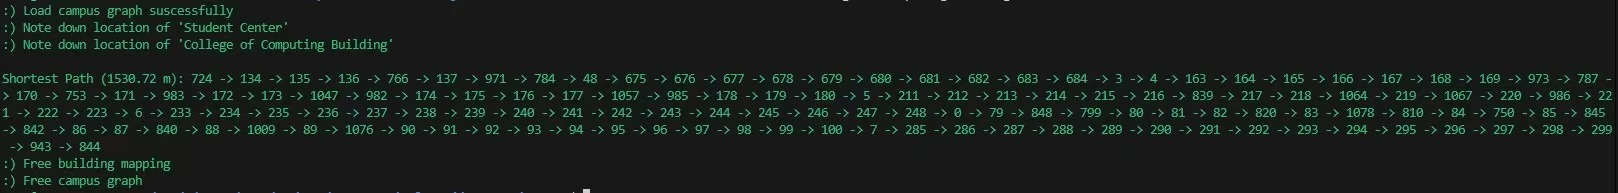
\includegraphics[width=1.0\textwidth]{initialResult.jpg}
\caption{The computed path from Student Center (724) to College of Computing (844).}
\end{figure}

% Last Page

\section*{Acknowledgment \& Upcoming Work Distribution}

We thank the Georgia Tech CSE 6010 teaching staff for their guidance during the early stages of this project.  
The current implementation and progress can be found at our \href{https://github.com/fredkyang/cse6010-buzznav}{GitHub repository}, which is intended solely for use in CSE 6010 (Fall 25) coursework.

In the future, we will divide the tasks among members as below:
\begin{itemize}
    \item \textbf{Algorithm \& Core Functionality}: Fred Yang, Jing He, Chia-Hsin Chiu
        \begin{itemize}
            \item implement Dijkstra's algorithm for comparison (runtime and path results).
            \item Polish A* algorithm
            \item Add simple performance logging
        \end{itemize}
    \item \textbf{Data Handling \& Graph Extensions}: Haowen Jiang, Jing He, Ming-Cheng Fan
        \begin{itemize}
            \item Improve CSV parsing robustness (e.g. check invalid edges).
            \item Integrate building entrance coordinates more accurately.
            \item Add location nodes other than buildings, such as statues, printers, restrooms, parking lot, etc.
        \end{itemize}
    \item \textbf{Routing Output \& Instructions}: Fred Yang, Ming-Cheng Fan, Haowen Jiang
        \begin{itemize}
            \item Implement turn-by-turn instruction for navigation system
            \item Format clearly results for users (expected to print clear instruction text instead of nodes\_id).
        \end{itemize}
    \item \textbf{Front-End UI}: Fred Yang, Chia-Hsin Chiu, Ming-Cheng Fan
        \begin{itemize}
            \item Build a user-friendly web that allows users to interact with our BuzzNav system via visualized map.
            \item Allow users to interactively filter and locate points of interest.
        \end{itemize}
    \item \textbf{Testing, Integration \& GitHub Repository Maintenance}: Team-wide
\end{itemize}

%\bibliographystyle{unsrt}
%\bibliography{references}

\end{document}